\documentclass[10pt, a4paper, twocolumn]{article}

\usepackage{amsmath, amsthm, amssymb}
\usepackage[top=0.7in, bottom=0.75in, left=0.65in, right=0.65in, columnsep=0.25in]{geometry}
\usepackage{graphicx}
\usepackage{booktabs}
\usepackage{hyperref}
\usepackage{caption}

\captionsetup{font=footnotesize, labelfont=bf, skip=3pt}

\newtheorem{theorem}{Theorem}
\newtheorem{proposition}{Proposition}
\newtheorem{assumption}{Assumption}
\newtheorem{remark}{Remark}

\title{\vspace{-1.2em}\Large\textbf{Resilient I-Bug Navigation under Intermittent Signal Spoofing}}

\author{
  \textbf{Tsuriel Vizel} \quad \textbf{Avraham Guez} \\
  \small Supervisor: Dr.\ Andrey Zhitnikov \\
  \small Technion -- Israel Institute of Technology \\
  \vspace{-1.2em}
}
\date{}

\begin{document}

\maketitle

\begin{abstract}
\noindent
Minimalist autonomous robots operating in GPS-denied environments rely on local sensor feedback rather than global coordinates or odometry. The I-Bug algorithm achieves provable target convergence using only a contact sensor and a scalar signal-intensity sensor. However, in noncoherent sensing settings where the receiver observes additive contributions from multiple emitters, intensity-based navigation is acutely vulnerable to intermittent adversarial spoofing. An additive spoofing transmitter warps the spatial intensity gradient in free space and injects false maxima along obstacle boundaries, trapping standard I-Bug agents in perpetual loops. We present a kinematics-based temporal anomaly filter and two counter-strategies—a \textit{Cautious} strategy that conditionally preserves the convergence guarantee of benign I-Bug under our threat model, and a low-latency \textit{Inertial} heuristic—requiring zero additional hardware. We prove a conditional preservation theorem showing that under intermittent step-spoofing (Assumptions~1--2), the Cautious strategy preserves the exact active-state spatial trajectory of any converging benign I-Bug execution, and we prove that freezing memory alone while continuing deterministic boundary motion is insufficient for universal convergence due to topological phase-locking (resonance). Paired evaluations across $1,000,000$ randomized 2D obstacle environments show that under the sampled environment distribution, the unmodified Naive I-Bug baseline succeeds in only $54.68\% \pm 0.10\%$ of runs, the Inertial heuristic achieves $99.61\% \pm 0.01\%$ success while reducing mean steps among successful runs by $20.5\%$, and the Cautious strategy achieves a $100.00\%$ observed success rate ($95\%$ Clopper--Pearson CI: $[99.9996\%, 100.00\%]$), matching the no-attack I-Bug reference.
\end{abstract}

\section{Introduction and Threat Model}
Classical Bug navigation provides convergence guarantees in unknown planar environments using limited local sensing \cite{lumelsky1987path, kamon1998tangentbug}, while the I-Bug algorithm replaces coordinate and range information with target-signal intensity \cite{taylor2009ibug, taylor2014intensity}. At this theoretical limit of sensory minimalism, a disk-shaped robot of radius $r_c > 0$ navigates a bounded planar workspace $\mathcal{W} \subset \mathbb{R}^2$ containing unknown, piecewise-analytic obstacles $\mathcal{O} = \{O_1, \dots, O_M\}$ (with collision-free configuration space $\mathcal{F} \subset \mathcal{W}$) using only a local contact bumper and a scalar sensor measuring emission intensity from an unknown target beacon $p_t \in \mathcal{F}$.

In benign conditions, the target intensity is a strictly decreasing radial function of Euclidean distance, $m(p - p_t) = \|p - p_t\|_2^{-1}$, and the mission succeeds when $\|p - p_t\|_2 < R_{\text{reach}}$. Without coordinates or odometry, the robot executes three primitives at discrete control steps $k \in \mathbb{N}_0$ (step period $\Delta t$, step size $\Delta s = v_{\max}\Delta t$):
\begin{enumerate}
    \item $u_{\text{ori}}$ (\textbf{Orient}): Aligns heading $\theta_k$ with a local gradient-direction estimate obtained from spatially local queries of the same scalar intensity sensor $S(p, t)$:
    \begin{equation}
        \theta_{\nabla}(p, t) = \operatorname{atan2}\!\bigl(\partial_y S(p, t),\, \partial_x S(p, t)\bigr) \pmod{2\pi}.
        \label{eq:grad_angle}
    \end{equation}
    This realizes the I-Bug orientation primitive without an additional sensor: in simulation, the derivatives are central finite differences of $S$ at four nearby probe points within one control step (we assume $u(t)$ does not switch during the probes).
    \item $u_{\text{fwd}}$ (\textbf{Move Forward}): Steps linearly along $\theta_k$ while in free-space state \texttt{MoveToTower}. Upon obstacle contact, it records threshold $i_H \leftarrow \max(S(p_k, t_k), i_H)$, turns right by $\pi/2$, and enters \texttt{FollowObstacle}.
    \item $u_{\text{fol}}$ (\textbf{Follow Boundary}): Tracks the obstacle perimeter keeping the wall on its left while updating the local boundary maximum $i_{\text{max}}$. Once $i_{\text{max}} > i_H + \epsilon$ followed by a descending sample $S(p_k, t_k) < i_{\text{max}} - \epsilon$, it updates $i_H \leftarrow i_{\text{max}}$, applies $u_{\text{ori}}$, and returns to \texttt{MoveToTower}.
\end{enumerate}

\noindent\textbf{Adversarial Additive RSS Model.}
Spoofed navigation signals can manipulate autonomous platforms, while sophisticated attackers may employ intermittent or covert signal takeover to disrupt guidance \cite{kerns2014unmanned, psiaki2016gnss}. Consider a malicious transmitter at an unknown location $p_e \in \mathcal{F}$ broadcasting an intermittent spoofing signal of strength $\alpha_e > 0$ governed by switching indicator $u(t) \in \{0, 1\}$.

\begin{assumption}[Additive RSS Superposition Field]
\label{assump:superposition}
We study an incoherent additive received-signal-strength (RSS) abstraction in which the sensor reports the sum of the legitimate and adversarial source contributions at position $p \in \mathcal{F}$ and time $t \ge 0$:
\begin{equation}
    S(p, t) = m(p - p_t) + e(p, t), \quad e(p, t) = u(t)\,\frac{\alpha_e}{\|p - p_e\|_2}.
    \label{eq:superposition}
\end{equation}
\end{assumption}

When $u(t) = 1$, $e(p, t)$ corrupts both the scalar reading $S(p, t)$ and its spatial gradient:
\begin{equation}
    \nabla_p S(p, t) = -\frac{p - p_t}{\|p - p_t\|_2^3} - u(t)\,\alpha_e \frac{p - p_e}{\|p - p_e\|_2^3}.
    \label{eq:corrupted_grad}
\end{equation}
Thus, an unprotected robot is deflected off course during $u_{\text{ori}}$ and records poisoned hit thresholds $i_H$ during obstacle contact that cannot be satisfied once $u(t) \to 0$, trapping the robot in infinite boundary-following loops.

\section{Physics-Informed Anomaly Detection and Counter-Strategies}

Motivated by physics-based attack detection \cite{giraldo2018survey} and classical abrupt-change detection \cite{basseville1993detection}, we defend the robot without additional hardware or oracle access to $m(p - p_t)$ by exploiting the separation between bounded motion-induced variation and discontinuous transmitter switching.

\begin{assumption}[Kinematic Lipschitz Bound vs.\ Temporal Discontinuity]
\label{assump:discontinuity}
Over a high-rate sensor sampling interval $\delta t \ll \Delta t$ (maximum displacement $\delta s = v_{\max}\delta t \ll R_{\text{reach}}$) during which the adversary is inactive ($u \equiv 0$), the natural intensity variation from reference $I_{\text{ref}} = m(p - p_t) = 1/d$ is bounded by the local radial Lipschitz increment:
\begin{equation}
    \Delta I_{\max}(I_{\text{ref}}) = \frac{\delta s}{d(d - \delta s)} = \frac{\delta s\, I_{\text{ref}}^2}{1 - \delta s\, I_{\text{ref}}}.
    \label{eq:lipschitz}
\end{equation}
Conversely, $u(t)$ switches between $0$ and $1$ such that every active burst lasts at most $T_{\text{on}} \ge 1$ steps and every inactive interval lasts at least $T_{\text{off}} > N_{\text{confirm}}$ steps (a fixed-period schedule is a special case), producing an instantaneous step jump
\begin{equation}
    e_{\min} := \frac{\alpha_e}{\max_{p \in \mathcal{F}_{\text{nav}}} \|p - p_e\|_2} \ge \frac{\alpha_e}{\operatorname{diam}(\mathcal{W})}
    \label{eq:emin_short}
\end{equation}
that satisfies $e_{\min} > \eta_{\text{spike}} \max_{p \in \mathcal{F}_{\text{nav}}} \Delta I_{\max}(m(p-p_t))$.
\end{assumption}

\begin{remark}[Physical Motivation, Scope \& Bounded Noise]
Assumption~\ref{assump:discontinuity} is motivated by time-scale separation: electronic sampling ($\text{kHz}$) is orders of magnitude faster than mechanical translation ($v_{\max}$), making $\delta s = v_{\max}\delta t$ and $\Delta I_{\max}$ small relative to switching transients. The guarantee excludes continuously active, slowly ramped, or sub-threshold attacks whose temporal residual remains below the detection threshold \cite{psiaki2016gnss}; formal analysis of such stealthy or near-field attacks is left for future work. In particular, a defense-aware adversary can stall the Cautious robot indefinitely (denial of service) by keeping $u(t) = 1$ or switching off for at most $N_{\text{confirm}}$ steps; Theorem~\ref{thm:cautious} guarantees safety, not liveness, against such attackers. Under bounded noise $|\nu_k| \le \varepsilon_{\text{noise}}$, false positives are excluded if $\Delta I_{\max} + 2\varepsilon_{\text{noise}} < \eta_{\text{spike}}\Delta I_{\max}$, and false negatives are excluded if $e_{\min} - 2\varepsilon_{\text{noise}} > \eta_{\text{spike}}\Delta I_{\max}$ (and analogously for $\mathcal{A}_{\text{drop}}$ with $\eta_{\text{drop}} \le \eta_{\text{spike}}$).
\end{remark}

\noindent\textbf{Anomaly Filter.}
At the start of step $k$ (before actuation), the filter compares the pre-step reading $I_k^- = S(p_{k-1}, t_k)$ against the previous post-step reading $I_{k-1}^+ = S(p_{k-1}, t_{k-1})$. Note that at an activation transition ($0 \to 1$), $I_{k-1}^+ = m(p_{k-1}-p_t)$ is uncorrupted, whereas at a deactivation transition ($1 \to 0$), $I_k^- = m(p_{k-1}-p_t)$ is uncorrupted. With $\Delta I_k = I_k^- - I_{k-1}^+$, positive (\textit{spike}) and negative (\textit{drop}) anomalies are flagged via:
\begin{align}
    \mathcal{A}_{\text{spike}} &\iff \Delta I_k > \eta_{\text{spike}}\,\Delta I_{\max}(I_{k-1}^+), \label{eq:spike} \\
    \mathcal{A}_{\text{drop}} &\iff (-\Delta I_k > 0.15 I_{k-1}^+) \;\lor \nonumber\\
    &\qquad\quad (-\Delta I_k > \eta_{\text{drop}}\Delta I_{\max}(I_k^-)), \label{eq:drop}
\end{align}
where $\eta_{\text{spike}} = 2.0$ and $\eta_{\text{drop}} = 1.2$. Both readings are taken at the same position $p_{k-1}$, so the benign $\Delta I_k$ is exactly zero in our noiseless simulation; $\Delta I_{\max}$ is a conservative margin for physical sensors that integrate over $\delta t$ while moving up to $\delta s$, and for noise (Remark~1). The $15\%$ term is a heuristic safeguard that only adds detections and is not used by the analysis. To the best of our knowledge, we are not aware of a prior anti-spoofing mechanism designed specifically for the minimalist I-Bug framework; we evaluate three strategies:
\begin{itemize}
    \item \textbf{Naive (Original I-Bug Baseline \cite{taylor2014intensity}):} Bypasses the filter, executing $u_{\text{ori}}, u_{\text{fwd}}, u_{\text{fol}}$ and updating $i_H$ directly on $S(p, t)$.
    \item \textbf{Cautious (State-Freezing):} Upon $\mathcal{A}_{\text{spike}}$, the robot enters \texttt{Paused} mode: it commands zero velocity ($\Delta p_k = 0$), locks its pose $(p_{\text{frozen}}, \theta_{\text{frozen}})$ and internal memory $(i_H, i_{\text{max}}, i_{\text{mem}})$, and waits until $\mathcal{A}_{\text{drop}}$ is observed and confirmed over $N_{\text{confirm}} = 3$ consecutive stable steps before resuming \texttt{Normal} closed-loop navigation.
    \item \textbf{Inertial (Open-Loop Heuristic):} Upon $\mathcal{A}_{\text{spike}}$, the robot enters \texttt{InertialMode}: it freezes its heading $\theta_{\text{frozen}}$ and suspends memory/peak updates, but continues moving. In \texttt{MoveToTower}, it suppresses $u_{\text{ori}}$ and steps forward linearly via $u_{\text{fwd}}$ (initializing $i_H \leftarrow i_{\text{mem}}$ from its last clean memory if an obstacle is hit while blind). In \texttt{FollowObstacle}, it continues perimeter tracking via $u_{\text{fol}}$ while suspending the leave-obstacle check until $\mathcal{A}_{\text{drop}}$ restores \texttt{Normal} mode.
\end{itemize}

\section{Formal Convergence \& Resonance Analysis}

\begin{theorem}[Conditional Active-State Trajectory and Convergence Preservation]
\label{thm:cautious}
Under Assumptions~\ref{assump:superposition} and~\ref{assump:discontinuity} with $\eta_{\text{drop}} \le \eta_{\text{spike}}$ and $T_{\text{off}} > N_{\text{confirm}}$, for any workspace $\mathcal{W}$ and benign field $m$:
(i) after removing the paused steps, the sequence of poses and internal states of the Cautious robot coincides step-by-step with the benign baseline I-Bug execution $\gamma_{\text{ideal}}$; and
(ii) whenever the benign execution reaches $\|p_k - p_t\|_2 < R_{\text{reach}}$ in $N_{\text{ideal}} < \infty$ active steps (in particular, under the convergence assumptions of \cite{taylor2014intensity}), the Cautious robot reaches the target in at most
\begin{equation}
    N_{\text{cautious}} \le N_{\text{ideal}} + \left\lceil \frac{N_{\text{ideal}}}{T_{\text{off}} - N_{\text{confirm}}} \right\rceil (T_{\text{on}} + N_{\text{confirm}})
    \label{eq:bound}
\end{equation}
finite steps.
\end{theorem}

\begin{proof}
At every adversarial activation step $k_j^{\text{on}}$, $\Delta I_k = m_e(p_{k-1} - p_e) \ge e_{\min} > \eta_{\text{spike}}\Delta I_{\max}(I_{k-1}^+)$, triggering $\mathcal{A}_{\text{spike}}$ prior to actuation or memory modification. Throughout $[k_j^{\text{on}}, k_j^{\text{off}}-1]$, $p_k$ is stationary and $\Sigma_k = (p_k, \theta_k, \text{mode}, i_H, i_{\text{max}}, i_{\text{mem}})$ remains locked. At $k_j^{\text{off}}$, since $\eta_{\text{drop}} \le \eta_{\text{spike}}$, the drop $-m_e(p_{k-1}-p_e) \ge e_{\min} > \eta_{\text{drop}}\Delta I_{\max}(I_{k_j^{\text{off}}}^-)$ triggers $\mathcal{A}_{\text{drop}}$, and after $N_{\text{confirm}}$ stationary verification ticks with $u(t)=0$, the robot resumes at $k_j^{\text{res}} = k_j^{\text{off}} + N_{\text{confirm}} - 1$ with $\Sigma(k_j^{\text{res}}) = \Sigma(k_j^{\text{on}} - 1)$. Consequently, during every active step $\tau$, $u(t_k) = 0 \implies S(p, t_k) = m(p - p_t)$ and $\nabla_p S = \nabla_p m$. By induction on active steps $\tau$, $\Sigma(\tau) \equiv \Sigma_{\text{ideal}}(\tau)$, so the active-step subsequence of $\gamma_{\text{cautious}}$ equals $\gamma_{\text{ideal}}$. Whenever $\gamma_{\text{ideal}}$ converges in $N_{\text{ideal}} < \infty$ steps, each switching cycle yields at least $T_{\text{off}} - N_{\text{confirm}} \ge 1$ active steps for at most $T_{\text{on}} + N_{\text{confirm}}$ paused steps, establishing Eq.~\eqref{eq:bound}.
\end{proof}

\begin{proposition}[Insufficiency of Memory Freezing Alone]
\label{prop:resonance}
Freezing internal memory alone while continuing deterministic boundary motion is insufficient to guarantee universal convergence. Let $\mathcal{A}_L \subset \partial O_i$ denote the boundary departure-detection arc over which the leave-event sequence (climb above $i_H + \epsilon$, peak $i_{\max}$, and descent by $\epsilon$) must be evaluated on an obstacle $O_i$ of perimeter $L_i$. If the orbital period $T_{\text{orbit}} = L_i / (v_{\text{fol}}\Delta t)$ satisfies $T_{\text{orbit}} = m\,T_{\text{cycle}}$ ($m \in \mathbb{N}$) and the blind arc of length $v_{\text{fol}} T_{\text{on}}\Delta t$ during $[k_j^{\text{on}}, k_j^{\text{off}})$ covers $\mathcal{A}_L$, the Inertial robot will bypass $\mathcal{A}_L$ while peak detection is suspended on every subsequent revolution, trapping it in an infinite limit cycle (while near-commensurate periods $T_{\text{orbit}} \approx m\,T_{\text{cycle}}$ induce prolonged finite trapping).
\end{proposition}

\section{Large-Scale Empirical Evaluation}
We implemented a continuous 2D kinematic simulator in Julia ($\mathcal{W} = [0, 20]^2$, $p_0 = (2, 1)$, $p_t = (18, 18)$, $R_{\text{reach}} = 0.5$, $r_c = \Delta s = 0.3$, $T_{\text{cycle}} = 40$, $T_{\text{on}} = 10$, $\alpha_e = 1.0$, horizon $N_{\max} = 2,000$, filter $\delta s = 0.002$). The transmitter $p_e$ is sampled uniformly in free space with $\|p_e - p_0\|_2 > 6$, $\|p_e - p_t\|_2 > 8$, and follows a fixed schedule ($T_{\text{on}} = 10$, $T_{\text{off}} = 30$, first activation at step $20$). Across $1,000,000$ procedurally generated mazes (10--16 overlapping rectangular walls with wide collision-free passages and perimeter margins), all three strategies were evaluated in paired trials, plus a no-attack ($u \equiv 0$) benign I-Bug reference on the same mazes (under $u \equiv 0$, Naive, Cautious, and Inertial produce identical step counts in $100\%$ of runs, confirming zero false positives).

\begin{table}[htbp]
\centering
\scriptsize
\setlength{\tabcolsep}{2.2pt}
\vspace{-0.4em}
\caption{Paired Evaluation ($10^6$ Runs; Step Stats on Succ.\ vs.\ Capped All)}
\label{tab:results}
\resizebox{\linewidth}{!}{%
\begin{tabular}{@{}lcccc@{}}
\toprule
\textbf{Strategy} & \textbf{Success ($95\%$ CI)} & \textbf{Mean (Succ.)} & \textbf{Med.\ [IQR] (Succ.)} & \textbf{$\bar{N}_{\text{capped}}$} \\ \midrule
\textit{Benign I-Bug (no attack)} & \textit{$100.00\%$} & \textit{$132.6$} & \textit{$126.0$ $[108,\, 150]$} & \textit{$132.6$} \\ \midrule
Naive \cite{taylor2014intensity} & $54.68\% \pm 0.10\%$  & $199.3$ & $153.0$ $[121,\, 205]$ & $1015.4$ \\
Cautious & $\mathbf{100.00\%}$ ($[99.9996, 100]$) & $193.0$ & $178.0$ $[160,\, 215]$ & $193.0$ \\
Inertial & $99.61\% \pm 0.01\%$  & $\mathbf{153.4}$ & $\mathbf{135.0}$ $[115,\, 168]$ & $\mathbf{160.6}$ \\ \bottomrule
\end{tabular}%
}
\vspace{-1.2em}
\end{table}

\noindent\textbf{Results and Conclusion.}
Table~\ref{tab:results} and Fig.~\ref{fig:trap} corroborate our theoretical findings under the sampled environment distribution:
(1) The unmodified \textit{Naive} I-Bug baseline fails in $45.32\%$ of the sampled environments, with representative failures exhibiting gradient deflection and threshold poisoning (e.g., $i_H = 1.230$ in Fig.~\ref{fig:trap}).
(2) Under Assumptions~\ref{assump:superposition}--\ref{assump:discontinuity}, the \textit{Cautious} strategy achieves an observed $100.00\%$ success rate ($10^6 / 10^6$ runs, maximum observed completion time of $578$ steps; $137$ steps in Fig.~\ref{fig:trap}), corroborating Theorem~\ref{thm:cautious}. Since benign I-Bug also succeeds in every maze, this shows \emph{preservation} rather than improvement: Cautious succeeds exactly where benign I-Bug does, satisfies Eq.~\eqref{eq:bound} in every run, and pays a mean overhead of $60.4$ steps ($+45.6\%$).
(3) Among successful runs, the \textit{Inertial} heuristic reduces mean completion steps by $20.5\%$ ($153.4$ vs.\ $193.0$ steps; and by $16.8\%$ under the unconditional horizon-capped metric $\bar{N}_{\text{capped}} = 160.6$), while failing in $0.39\%$ ($3,877$) of trials; its observed failures are consistent with the phase-locking mechanism of Proposition~\ref{prop:resonance}, as illustrated in Fig.~\ref{fig:trap} ($i_H = 0.167$). This establishes a clear security-efficiency trade-off: full state-and-motion freezing conditionally preserves benign I-Bug convergence under intermittent step-spoofing (Remark~1), whereas open-loop continuation maximizes speed when rare resonance traps are tolerable or mitigated via stochastic excitation.

\begin{figure}[htbp]
    \centering
    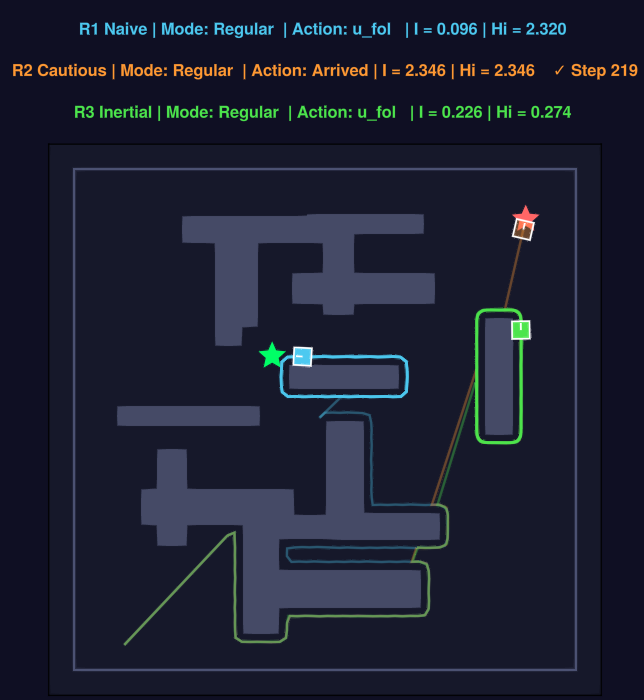
\includegraphics[width=0.55\linewidth]{simulation_trap.png}
    \caption{Representative double failure: Naive is threshold-poisoned at the L-obstacle; Inertial enters a phase-locked boundary loop; Cautious pauses during spoofing and reaches the target.}
    \label{fig:trap}
    \vspace{-0.8em}
\end{figure}

\begin{thebibliography}{8}
\footnotesize
\setlength{\itemsep}{0pt}
\bibitem{lumelsky1987path}
V.~J. Lumelsky and A.~A. Stepanov, ``Path-planning strategies for a point mobile automaton moving amidst unknown obstacles of arbitrary shape,'' \textit{Algorithmica}, vol.~2, no.~1, pp.~403--430, 1987.

\bibitem{kamon1998tangentbug}
I.~Kamon, E.~Rimon, and E.~Rivlin, ``TangentBug: A range-sensor-based navigation algorithm,'' \textit{Int. J. Robot. Res.}, vol.~17, no.~9, pp.~934--953, 1998.

\bibitem{taylor2009ibug}
K.~Taylor and S.~M. LaValle, ``I-Bug: An intensity-based bug algorithm,'' in \textit{Proc. IEEE Int. Conf. Robot. Autom. (ICRA)}, 2009, pp.~3981--3986.

\bibitem{taylor2014intensity}
K.~Taylor and S.~M. LaValle, ``Intensity-based navigation with global guarantees,'' \textit{Auton. Robots}, vol.~36, no.~4, pp.~349--364, 2014.

\bibitem{kerns2014unmanned}
A.~J. Kerns, D.~P. Shepard, J.~A. Bhatti, and T.~E. Humphreys, ``Unmanned aircraft capture and control via GPS spoofing,'' \textit{J. Field Robot.}, vol.~31, no.~4, pp.~617--636, 2014.

\bibitem{psiaki2016gnss}
M.~L. Psiaki and T.~E. Humphreys, ``GNSS spoofing and detection,'' \textit{Proc. IEEE}, vol.~104, no.~6, pp.~1258--1270, 2016.

\bibitem{giraldo2018survey}
J.~Giraldo \textit{et al.}, ``A survey of physics-based attack detection in cyber-physical systems,'' \textit{ACM Comput. Surv.}, vol.~51, no.~4, Art.~no.~76, pp.~1--36, 2018.

\bibitem{basseville1993detection}
M.~Basseville and I.~V. Nikiforov, \textit{Detection of Abrupt Changes: Theory and Application}. Englewood Cliffs, NJ, USA: Prentice Hall, 1993.
\end{thebibliography}

\end{document}
